\section{7. Se\~nal de televisi\'on en Argentina}

El sistema de codificacion utilizado en la transmisión de señales de televisión analógica a color en la Argentina es el sistema PAL-N o l\'inea de fase alternada, por sus siglas en ingl\'es. El sistema PAL surgió en el año 1963, de manos del Dr. Walter Bruch en los laboratorios de Telefunken en su intento por mejorar la calidad y reducir los defectos en los tonos de color que presentaba el sistema NTSC. El ancho de banda total de un canal de televisión es de $6 MHz$ y dado que justamente se trata de una señal televisiva existen dos portadoras, una de sonido $4,5 MHz$ por encima del valor base y otra de color $3.582056 MHz$ sobre el balor de frecuencia de referencia. El nombre phase alternating line  hace referencia al modo en que la información de crominancia (color) de la señal de vídeo es transmitida, siendo invertida en fase en cada línea, permitiendo la corrección automática de los posibles errores en fase al cancelarse entre sí. Aprovechando que habitualmente el contenido de color de una línea y la siguiente es similar, en el receptor se compensan automáticamente los errores de tono de color tomando para la muestra en pantalla el valor medio de una línea y la siguiente, dado que el posible error de fase existente entre ambas será contrario. De esta forma, en lugar de apreciarse dicho error como un corrimiento del tono, se aprecia como un ligero defecto de saturación de color, que es mucho menos perceptible al ojo humano.\newline


Utilizando el analizador de espectro se logró escuchar la señal de audio del canal 9 a una frecuencia de $191.7 MHz$ o $5,7MHz$ por sobre la frecuencia de referencia lo cual concuerda con los datos proveídos por la ENACOM, pero es mayor a los $4,5MHz$ mencionados anteriormente. Debido que en realidad se asignan una banda de frecuencias sobre en la cual el canal puede emitir, los resultados son satisfactorios. 


\begin{figure}[H]
    \centering
    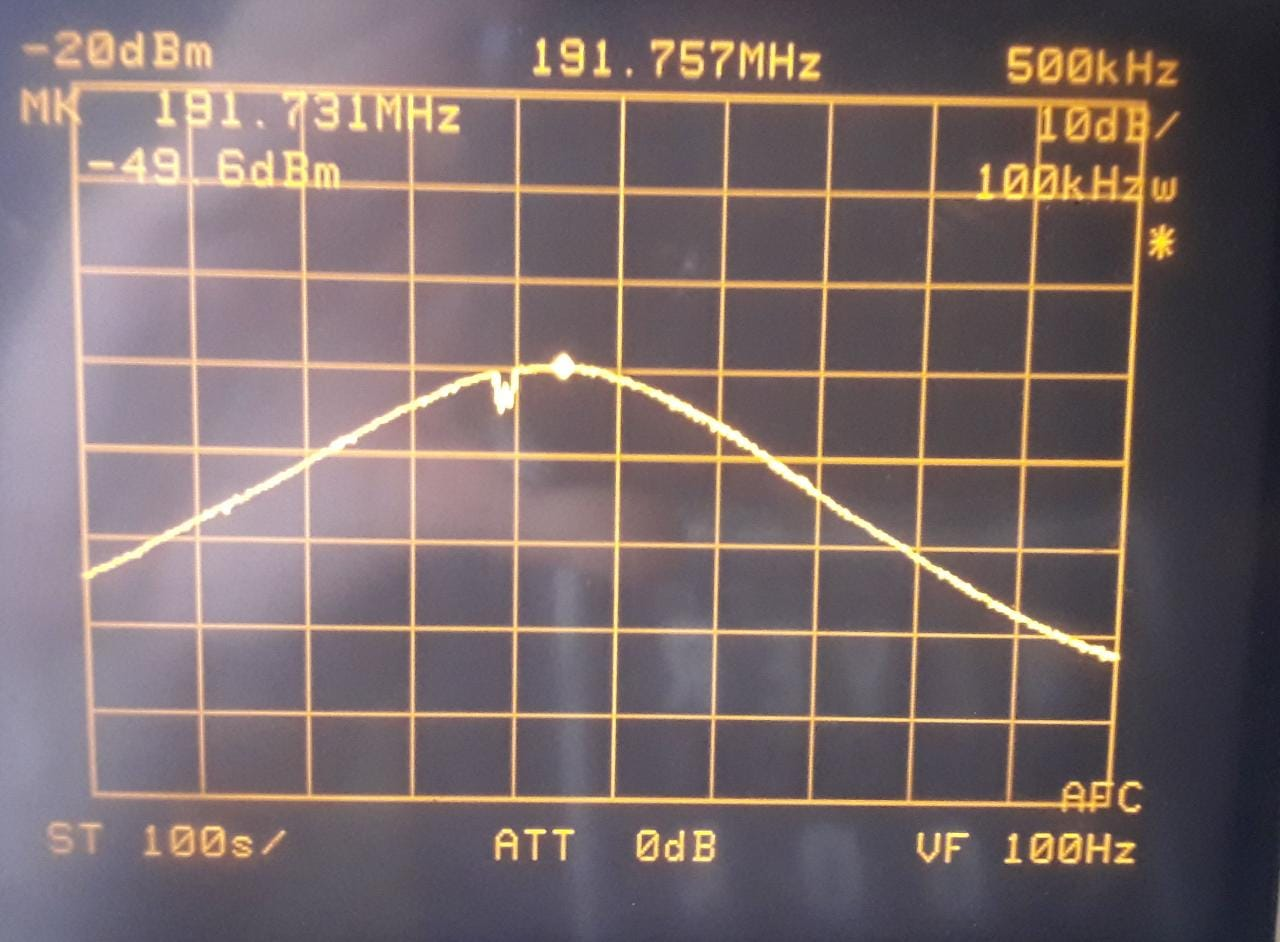
\includegraphics[scale=0.3]{Recursos/Canal9.jpeg}
    \caption{Emisión de sonido canal 9}
\end{figure}


